%%%%%%%%%%%%%%%%%%%%%%%%%%%%%%%%%%%%%%%%%%%%%%%%%%%%%%%%%%%%%%%%%%%%%%%%%%%%%
%%% LaTeX-Rahmen fuer das Erstellen von Bachelorarbeiten
%%%%%%%%%%%%%%%%%%%%%%%%%%%%%%%%%%%%%%%%%%%%%%%%%%%%%%%%%%%%%%%%%%%%%%%%%%%%%

%%%%%%%%%%%%%%%%%%%%%%%%%%%%%%%%%%%%%%%%%%%%%%%%%%%%%%%%%%%%%%%%%%%%%%%%%%%%%
%%% allgemeine Einstellungen
%%%%%%%%%%%%%%%%%%%%%%%%%%%%%%%%%%%%%%%%%%%%%%%%%%%%%%%%%%%%%%%%%%%%%%%%%%%%%

\documentclass[twoside,12pt,a4paper]{report}
%\usepackage{reportpage}
\usepackage{amsmath,amsfonts,amssymb,amsthm}
\usepackage{mathtools}
\usepackage{commath}
\usepackage{svg}

%\usepackage{epsf,german}
%\usepackage{natbib}
%\usepackage[natbibapa]{apacite}
\usepackage{apacite}
\usepackage{graphics, graphicx}
\usepackage{subcaption, framed, tcolorbox}
\usepackage[utf8]{inputenc}
\usepackage{latexsym}
\usepackage{todonotes}
\usepackage[margin=10pt,font=small,labelfont=bf]{caption}

\textwidth 14cm
\textheight 22cm
\topmargin 0.0cm
\evensidemargin 1cm
\oddsidemargin 1cm
%\footskip 2cm
\parskip0.5explus0.1exminus0.1ex
\setlength{\parindent}{7mm}

\pagestyle{headings}

\sloppy

\begin{document}

%%%%%%%%%%%%%%%%%%%%%%%%%%%%%%%%%%%%%%%%%%%%%%%%%%%%%%%%%%%%%%%%%%%%%%%%%%%%
%%% hier steht die neue Titelseite 
%%%%%%%%%%%%%%%%%%%%%%%%%%%%%%%%%%%%%%%%%%%%%%%%%%%%%%%%%%%%%%%%%%%%%%%%%%%%
 
\begin{titlepage}
 \begin{center}
  {\LARGE University of T\"ubingen}\\
  {\large Faculty of Science \\
Departement of Biology\\
Cognitive Neuroscience \\[4cm]}
  {\huge Bachelorthesis in Cognitive Science\\[2cm]}
  {\Large\bf  Quantitative Modelling of \textit{Apteronotus leptorhynchus'} Anatomy \\[1.5cm]}
 {\large Jana Kr\"amer}\\[0.5cm]
\today\\[3cm]
\begin{center}{\small\bf Supervisor}\\[0.5cm]
{\large Prof. Dr. Hanspeter A. Mallot}\\
  {\footnotesize Cognitive Neuroscience, Faculty of Science\\
	University of T\"ubingen}	\end{center}
	
	
  \end{center}
\end{titlepage}

%%%%%%%%%%%%%%%%%%%%%%%%%%%%%%%%%%%%%%%%%%%%%%%%%%%%%%%%%%%%%%%%%%%%%%%%%%%%
%%% Titelr"uckseite: Bibliographische Angaben
%%%%%%%%%%%%%%%%%%%%%%%%%%%%%%%%%%%%%%%%%%%%%%%%%%%%%%%%%%%%%%%%%%%%%%%%%%%%

\thispagestyle{empty}
\vspace*{\fill}
\begin{minipage}{13.2cm}
\textbf{Krämer, Jana:}\\
\emph{Quantitative Modelling of} Apteronotus leptorhynchus' \emph{Anatomy}\\ 
Bachelorthesis in Cognitive Science\\
Eberhard Karls University T\"ubingen\\
Processing period: 20.11.2019-20.03.2020
\end{minipage}
\newpage

%%%%%%%%%%%%%%%%%%%%%%%%%%%%%%%%%%%%%%%%%%%%%%%%%%%%%%%%%%%%%%%%%%%%%%%%%%%%

\pagenumbering{roman}
\setcounter{page}{1}

%%%%%%%%%%%%%%%%%%%%%%%%%%%%%%%%%%%%%%%%%%%%%%%%%%%%%%%%%%%%%%%%%%%%%%%%%%%%
%%% Seite I: Zusammenfassug, Danksagung
%%%%%%%%%%%%%%%%%%%%%%%%%%%%%%%%%%%%%%%%%%%%%%%%%%%%%%%%%%%%%%%%%%%%%%%%%%%%
\section*{Zusammenfassung}
Aktive Elektrorezeption ist eine Sinneswahrnehmung, welche verschiedene Fischarten verwenden. Wozu genau die Fische sie nutzen, ist noch nicht gänzlich geklärt. Sicher ist zwar, dass sie mithilfe dieser Sinneswahrnehmung mit Artgenossen kommunizieren können, ob und bis in welches Detail sie in der Lage sind, Objekte damit zu erkennen, ist noch unbekannt. Um das herauszufinden, kann zum Beispiel ein in silico Modell des Fisches, seines elektrischen Feldes und der resultierenden Reaktion der Elektrorezeptoren implementiert werden. Der erste Teil, das Erstellen eines anatomischen Modells eines dieser Fische, des \textit{Apteronotus leptorhynchus}, ist das Thema dieser Bachelorarbeit. Dafür wurden paratransversale Schnitte durch den Fisch per MRT erfasst und jeweils über eine Simplex-Optimierung an eine ellipsenähnliche Funktion angenähert. Diese Querschnitte wurden dann entlang der Wirbelsäule,approximiert über eine Hyperbola, angeordnet. Veränderungen der Parameter dieser Hyperbola können einen abgeknickten Schwanz simulieren, da eine derartige Körperposition in einigen schwach elektrischen Fischen bei der Exploration ihrer Umgebung beobachtet wurde. Durch polynomielle Regressionen konnten im Anschluss kontinuierliche Werte für die Parameter der Funktion der Querschnitte bestimmt werden. Somit ist es schlussendlich möglich zu bestimmen, ob ein gegebener Punkt im Raum innerhalb oder außerhalb des Fisches liegt. Für Punkte innerhalb des Fisches wird zusätzlich noch bestimmt, ob sie Teil des elektrischen Organs, der Wirbelsäule oder des Rückenmarks sind. Das anatomische Modell des \textit{Apteronotus leptorhynchus} soll in Zukunft in ein allgemeines Modell integriert werden, welches auf Basis der genauen Daten besser verifizieren soll, wie detailliert der Fisch seine Umgebung durch die aktive Elektrorezeption wahrnehmen kann. 
\newpage

\section*{Abstract}

A not well understood type of perception, active electroreception, is present in some weakly electric fishes. They are using their electric sense to communicate with specimen. In contrast, it is not fully understood by now, if they are able to detect objects with it. To narrow this knowledge gap, an in silico model of a weakly electric fish, the \textit{Apteronotus leptorhynchus}, can be implemented. Such a model needs to include an approximation of the fish, its electric field and the response of its electroreceptors. Implementing the fish's anatomical model is the subject of this thesis. It is based on MRI data and the resulting paratransverse sectional data. Each section is approximated by an edited ellipsis that can have a tip at the ventral side. A polynomial regression over the necessary parameters then results in data for all paratransverse sections of the fish, not just for the discrete ones of the MRI sections. Positioning these approximated sections behind one another along the fish's backbone, that is modelled by a hyperbola, provides a sufficient fit and, thus, yields predicted points for all paratransverse sections. Additionally, the hyperbola's parameters may be changed such that the fish's tail is bent as this has been observed in exploration behaviour in other weakly electric fishes. The final implemented function then classifies a point as lying outside or inside the fish. If the latter is the case, it is tested for being positioned inside the fish's electric organ, the spinal chord or the backbone. In the future, this anatomical model will be included in a more general model that approximates the fish's whole electrosensory model to make it more accurate, which will further aid in understanding the evolutionary advantage of the electric sense. 

\newpage
\section*{Danksagung}

Vielen Dank an Thede Witschel, meinen Betreuer, der mir immer für Fragen zur Verfügung stand und mich geduldig unterstützt hat. Außerdem vielen Dank an Marc Weitz, der sich fast täglich meine Probleme angehört und versucht hat, mir bei ihrer Lösung zu helfen; und an meine Schwester, die mir bei allen mathematischen Fragestellung stets zur Verfügung stand. Und vielen Dank an alle KorrekturleserInnen für eure Anregungen und die Zeit, die ihr euch für mich genommen habt. 


%%%%%%%%%%%%%%%%%%%%%%%%%%%%%%%%%%%%%%%%%%%%%%%%%%%%%%%%%%%%%%%%%%%%%%%%%%%%%
%%% Inhaltsverzeichnis
%%%%%%%%%%%%%%%%%%%%%%%%%%%%%%%%%%%%%%%%%%%%%%%%%%%%%%%%%%%%%%%%%%%%%%%%%%%%%
\newpage
\renewcommand{\baselinestretch}{1.3}
\small\normalsize

\tableofcontents

\renewcommand{\baselinestretch}{1}
\small\normalsize



%%%%%%%%%%%%%%%%%%%%%%%%%%%%%%%%%%%%%%%%%%%%%%%%%%%%%%%%%%%%%%%%%%%%%%%%%%%%%
% Der Haupttext startet hier
%%%%%%%%%%%%%%%%%%%%%%%%%%%%%%%%%%%%%%%%%%%%%%%%%%%%%%%%%%%%%%%%%%%%%%%%%%%%%
\newpage
\pagenumbering{arabic}
\setcounter{page}{1}

%% Backbone
%%%%%%%%%%%%%%%%%%%%%%%%%%%%%%%%%%%%%%%%%%%%%%%%%%%%%%%%%%%%%%%%%%%%%%%%%%
% Information about Apteronotus Leptorhynchus 
%%%%%%%%%%%%%%%%%%%%%%%%%%%%%%%%%%%%%%%%%%%%%%%%%%%%%%%%%%%%%%%%%%%%%%%%%%

\chapter{Introduction} 
    \label{Introduction}
    
We, as human beings, hear sounds – the melody of a song, a rustle or a bang. We smell the aroma of coffee, the scent of cinnamon or the stench of foulness. We see the shape of an animal or the bright colour of the sun. We taste a fruit’s sweetness or the bitterness of drugs. We feel the rough surface of sandpaper or the heat of fire. But how does it feel, if there are irritations in the electric field around us? One cannot imagine how other types of perception feel, how accurate they are in terms of object detection, time or space. 

 Yet, other species use types of perception successfully that are unfamiliar to us. The most popular examples are probably bats and some whales that use echolocation to detect and locate objects. However, there are some less prominent examples as well, one of which is the central subject of this thesis: active electroception. It is present in different species but will be analysed in \textit{Apteronotus leptorhynchus}, a weak electric fish of the South American rivers. \textit{A. leptorhynchus}, was first recorded by Ellis in \citeA{eigenmann1905sternarchorhamphus} as \textit{Sternarchus leptorhynchus} and belongs to the order of Gymnotiformes. They share the electric sense only with the family of Mormyriformes, which are native to the rivers of Africa. Their most common ancestor did not possess an active electric sense and  the ancestors in between did neither. This separate evolution of the same system, called analogy, is what most likely happened for active electroception in Gymnotiformes and Mormyriformes. However, what drove active electroception to be advantegous for survival, remains unclear.
 
 To be able to understand this advantage, it is first necessary to understand its basic characteristics. Active electroception or electroreception results from weak electric organ discharges (EODs) released by the fish's electric organ, as the name already indicates. The description of the electroception as being active in this case refers to the self-generation of the EODs. 
To perceive the electric field that has been modified by the fish's surrounding area, there are tuberous electroreceptors spread through the fish's epidermis. They are specific to amplitude and phase of the electric signal \cite{assad1997electric}.

The signals perceived by the electroreceptors are thought to be used for two different functions: electrocommunication and electrolocation \cite{binder2009encyclopedia}. Electrocommunication is defined as being an information transfer between two electric fish based on their EODs. This includes, but is not limited to: Age, sex, individual identity and motivational state \cite{binder2009encyclopedia}. The presence and functionality of this communicative use of electroreception are relatively well studied \cite<e.g.>{fugere2010electric, bastian2001arginine, hupe2008electrocommunication} and seems to be used commonly by all weakly electric fish. In contrast, the presence and importance of electrolocation in \textit{A. leptorhynchus} is still under debate. Electrolocation, on the other hand, describes the detection of objects using distortions in the electric field and the resulting electroreceptors' responses \cite{binder2009encyclopedia}. Objects causing a reduction of the electric current flow are those with an impedance value higher than the water. The opposite effect, an increase of the electric current flow, results from objects with low impedance values \cite{bullock2006electroreception}. With that, it should be theoretically possible for the fish to receive some information about objects close-by.

Even if one assumes that the latter function is present as well, it is not obvious which advantage it brings to the animal processing the information. In which situations could electrolocation possibly be more informative than the visual information received? It has been suggested that the lack of sufficient light as present in turbid waters may lead to difficulties with the visual system. Therefore, electrolocation may be a useful replacement system to gain the necessary information \cite{assad1997electric}, although this hypothesis only holds if the species under research does live in areas with a lack of light. This is not the case for \textit{A. leptorhynchus} as they inhabitate mainly rivers with clear water that enables them to use their visual system appropriately. Other explanations have not yet been presented. Therefore, the advantage that may result from the evolution of electrolocation is not easily explained. One characteristic that needs to be taken into account though, is the nocturnal activity that \textit{A. leptorhynchus} show \cite{raab2019dominance}. The same is probably true for other species of Gymnotiformes \cite{kramer2009encyclopedia} and with that, there could be a connection in terms of evolution between the presence of the electric sense and the fish being nocturnal. 

To understand the processes underlying electrolocation it is necessary to conceive the evolutionary process that produced it. In particular, it contributes to differentiate between being an analogous development or just a by-product. That is the aim of the project, this thesis is part of: building an in silico model of \textit{A. leptorhynchus}. The model is meant to include the fish itself, its generated electric field and its electroreceptor's responses. The first part, the implementation of the fish's basic anatomy has been the goal of this thesis. The majority of models developed so far use very simple geometrical models of the fish's contour to approximate the acquired information \cite[among others]{bacher1983new, chen2005modeling}. \citeA{fujita2010modeling} modeled the fish's body shape even with a rectangle and both other mentioned papers did not put much attention to the shape. The study of \citeA{babineau2006modeling} has indicated, though, that the fish's body shape is essential for getting informative electroreceptors' responses. The authors compare two simple geometrical models to one describing \textit{A. leptorhynchus} contour more accurately. The latter one can account for the presence of most electroreceptors in the rostral region - the model leads to a smooth uniform electric field at exactly this location. However, Babineau et al. (2006) did not take into account the exact body contour of the fish. This is a necessary precondition to be able to model the electric field and the corresponding responses accurately. 

Following this line of research, we assumed that acquiring exact anatomical data of \textit{A. leptorhynchus} to base a model on, is the most reliable way to generate accurate data later on. Hence, we acquired an MRI scan of a recently expired specimen. The resulting sections through the fish's body were then used for the geometrical approximation of the body contour. The whole geometrical model is based on the backbone and is constructed relative to its position. Thus, the backbone is introduced first by a definition of a hyperbola that allows us to model the bending of the fish's tail. Secondly, the according Frenet coordinate frame at any point on the backbone was constructed to then place the cross-section within the according normal plane. The form of the cross-sections themselves was directly based on the MRI paratransverse sections. A parameterized ellipsis was edited such that a tip at its ventral side is possible to approximate the sections more accurately. Adding the information taken from the MRI data to the edited ellipses was done by applying a simplex optimization over 60 paratransverse sections. To get continuous data at any point on the backbone, a polynomial regression over the three parameters the ellipses were based on has been executed. With that, it is possible to generate the outer contour of the fish at any point on its backbone. The implementation of these steps leads to a function classifying a point given in space as being either on the inside or on the outside the fish. Furthermore, some inner parts of the fish were considered as well: its spinal chord, its backbone and its electric organ. The position of these parts was approximated relative to the backbone's center as well and points localized within one of them not only get the label 'inside' but 'spinal chord', 'backbone' or 'electric organ'. 
\cleardoublepage
%%%%%%%%%%%%%%%%%%%%%%%%%%%%%%%%%%%%%%%%%%%%%%%%%%%%%%%%%%%%%%%%%%%%%%%%%%
% Information about mathematical background on backbone and implementation
%%%%%%%%%%%%%%%%%%%%%%%%%%%%%%%%%%%%%%%%%%%%%%%%%%%%%%%%%%%%%%%%%%%%%%%%%%

\chapter{Modelling Background} 
    \label{Modelling background}
    
In this chapter, the theoretical background of the implementation as outlined in chapter \ref{implementation} is described. The chapter is divided in several sections that each describe the different steps of modelling the fish's anatomy. To prevent confusions about terms concerning positions across the fish's body, a definition of the fish's anatomical axes is introduced in paragraph \ref{axes}. Then, the description of the formalization of \textit{Apteronotus leptorhynchus'} anatomy follows. The first is to represent its backbone as a parameterised curve that forms either a straight line or a curve turned at one point by a given angle. This curve was the basis for the cross-sections which were placed perpendicular to the backbone. How this orthogonality was achieved, is described in detail in paragraph \ref{crosssectional planes}. The last paragraph, \ref{Cross sections}, deals with the form of the cross sections themselves, that were modelled with the sum of an ellipsis and a variation of the Lorenz curve.

\section{Definition of Anatomical Axes}
    \label{axes}
    
In general, one describes the anatomical position in vertebrates using three axes. Depending on the specific animal the terms describing these axes vary. Therefore, we want to define the terms for the planes of the fish's anatomy in this paragraph to avoid misunderstandings. 

We use the terminology suggested by \citeA{harder1976anatomy} illustrated in Figure \ref{fig:Axes}. The first plane and with that the first axis is the \textit{horizontal} plane. It divides the fish into a dorsal and a ventral part along the fish's long axis. Perpendicular to the horizontal axis is the \textit{median} plane that is also positioned along the fish's long axis. It is the only plane that divides the fish into two nearly symmetrical halves that may be termed \textit{left} and \textit{right} half, respectively. The last plane is positioned perpendicular to both other planes and is called the \textit{transverse} plane. It cuts the fish at the middle of the long axis into a \textit{cranial} and a \textit{caudal} part. \\

\begin{figure}
   \centering
   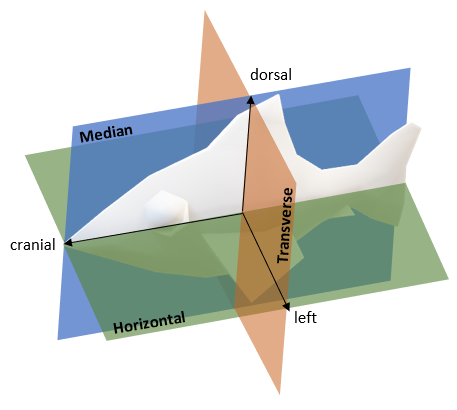
\includegraphics[width=10cm]{figures/Axes.PNG}
   \caption{Visualisation of a fish's axes. The median plane is depicted in blue, the horizontal plane in green and the transverse plane in red.}
   \label{fig:Axes}
\end{figure}

In the following chapters, various sections along one of the axes are used for the anatomical model. Their terminology is straightforward from the axes' terminology, but will be shortly defined here nevertheless: there are \textit{horizontal, median} and \textit{transverse} sections, respectively. Sections which are not positioned along one axis but rather parallel to it, are termed \textit{parahorizontal, paramedian} or \textit{paratransverse}. To shorten the term of the paratransverse section, that is used frequently in the following sections, we simply refer to them as \textit{cross-sections}.

\section{Backbone}
    \label{BackboneModelling}
    
The first step in modelling \textit{Apteronotus leptorhynchus'} anatomy consisted in modelling its backbone. This was done by describing a curve that can be, on the one hand, a straight line, if the fish does not bend its tail. And, on the other hand, bending should be possible, as specimen of \textit{Apteronotus leptorhynchus} do that to alter the spatial relation between their electric organ and their electroreceptors across the whole body \cite{bell1997generation}. Similar movements have been observed in \textit{Marcusenius cyprinoides} that belong to the family of Mormyriformes that also use active electrolocation as described in the introduction. Their exploration behaviour is visualized in Figure
\ref{ExplorationBehaviour} to get a more exact impression of the movements that were considered while modelling.

The horizontal coordinate, in the following represented by the $z$-coordinate, is kept constantly at $0$, because the fish does not move its body up- or downwards but keeps it rather straight or bent only in $x$- and $y$-direction, i.e. inside the plane spanned by transverse and median axis. 

\begin{figure}
   \centering
   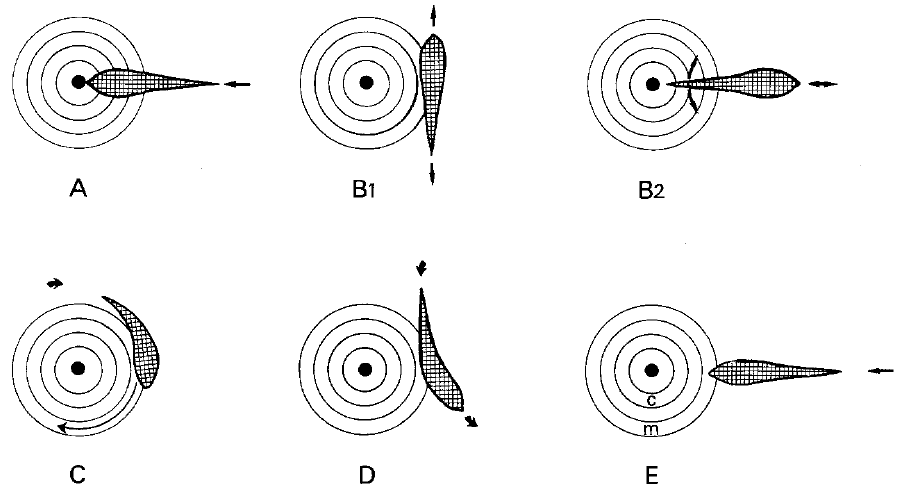
\includegraphics[width=10cm]{figures/ExplorationBehaviour.png}
   \caption{Exploration behaviour of \textit{Marcusenius cyprinoides} taken from \cite{toerring1979motor}. The different body shapes the fish uses in order to explore an object suggests, that an anatomical model of this species should provide various underlying backbone forms: as straight backbone and a curved one. If \textit{A. leptorhynchus} use the same behaviour, which is unknown by now, a model of this species' anatomy should offer the same possibilities. }
   \label{ExplorationBehaviour}
\end{figure}

A step-wise modulation of the fish's tail-bending behaviour is therefore necessary to model the temporally specific electric fields.
This was modelled with a curve that includes one turning point as this describes the fish's body position in a sufficient way. A hyperbola that suffices this criterion is visualized in Figure \ref{Backbonefunction}.
\begin{figure}[ht]
   \centering
   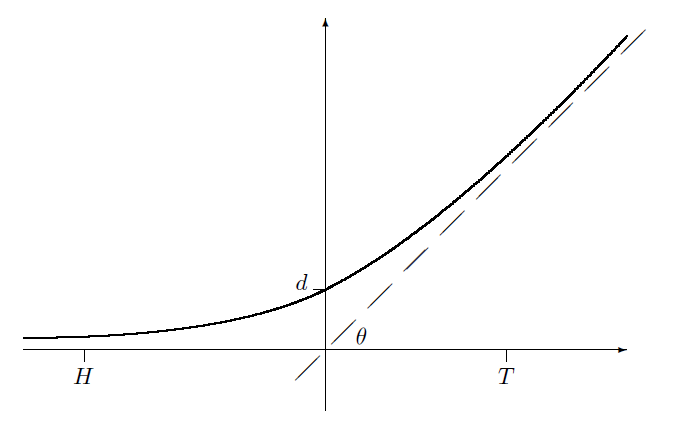
\includegraphics[width=10cm]{figures/BackboneFunction.PNG}
   \caption{The illustrated hyperbola models the fish's backbone as seen from above the fish, the horizontal axis is not visible. $H$ is the fish's head's transverse position, $T$ its tail's transverse position. $d$ specifies the median coordinate of the intersection between curve and median axis. The hyperbola converges to two asymptotes: The first one being the transverse axis, the second being a straight line from the origin with angle $\theta$ to the median axis.}
   \label{Backbonefunction}
\end{figure}

The hyperbola tends to two asymptotes at its limits. The first asymptote is the negative $x$-axis that represents the transverse axis while the other asymptote is given by a straight line with angle $0 \leq \theta < 90°$ from the $x$-axis. In the mathematical description of the hyperbola, the slope of the second asymptote is defined by $a := tan(\theta)$. The fish's head $H$ and due to that also the tail $T$ may be shifted along the $x$-axis to change the point at which the tail is bent, because the intersection with the y-axis (median axis), $d$, influences the curvature as well.
The equation for the hyperbola $f:\mathbb{R} \rightarrow \mathbb{R}$ is given by 
\begin{flalign}
f(x) = \frac{1}{2} \cdot (ax + \sqrt{4d^2 + a^2x^2}).
\end{flalign}

\newpage
To represent this equation in a parameterised planar curve depending only on the length parameter $l$, let $c: \mathbb{R} \rightarrow \mathbb{R}^2$ be:
\begin{flalign}
c(x) := \begin{pmatrix} x \\ f(x) \end{pmatrix}
\end{flalign}

Then one applies the general formula for the length of a parameterised curve as defined by \citeA[Def. 2.1.15]{bar2010elementare}
\begin{flalign}
l := \int_a^b{\norm{c'(x)} dx}
\end{flalign}
to $c$, with $H$ specified as the head's position. $c'(x)$ represents the first derivative of $c$. $s(b)$ then describes the length from the fish's head to the given transverse position $b$:
\begin{flalign}
l = s(b) = \int_H^b \sqrt{1+(f'(x))^2} dx.
\label{eq:s_x}
\end{flalign}

The parameterisation is necessary for further steps in modelling the fish's anatomy as described in the following paragraphs. 
Given a specific point $l$ on the backbone, its three-dimensional position is then described by $B(l): \mathbb{R} \rightarrow \mathbb{R}^3$:
\begin{flalign}
B(l) := \begin{pmatrix} s^{-1}(l) \\ f(s^{-1}(l)) \\ 0 \end{pmatrix}.
\label{eq:3dvector}
\end{flalign}

As mentioned before, the $z$-coordinate and with that the coordinate on the horizontal axis is kept constantly at $0$ because the fish does not move its body up- or downwards.

\section{Cross-sectional Planes}
    \label{crosssectional planes}
    
To be able to translate and turn the two-dimensional cross-sectional points resulting from the MRI data into three dimensions, it is first obligatory to define the Frenet-coordinate frame at each point along the backbone. Thus, the three vectors specifying the coordinate frame need to be defined in a general form depending on $l$, the point on the backbone. The tangent vector, $\vec{e_1}$, points along the fish's body axis, the normal vector, $\vec{e_2}$, points to its left and the binormal vector, $\vec{e_3}$, upwards. The $z$-coordinates of the hyperbola are kept constantly at $0$ and due to that the torsion $\tau$ as well. As a result, $\vec{e_3}$ is not dependent on $l$ and stays the same along the whole backbone. Following these characterestics, the unit Frenet vectors are given by
\begin{flalign}
\vec{e_1}(x) = \frac{c'(x)}{||c'(x)||}, \vec{e_2}(x) = \frac{\vec{e_1}'(x)}{||\vec{e_1}'(x)||}, \vec{e_3}(x) = \begin{pmatrix} 0 \\ 0 \\ 1 \end{pmatrix}. 
\end{flalign}

Using the definition of $B(l)$ from equation \ref{eq:3dvector}, that leads to
\begin{flalign}
\vec{e_1}(l) = \begin{pmatrix} 1 \\ f'(s^{-1}(l)) \\ 0\end{pmatrix} \cdot \frac{1}{||B'(l)||}
\end{flalign}

and
\begin{flalign}
\vec{e_2}(l) = \begin{pmatrix} f'(s^{-1}(l)) \\ -1 \\ 0\end{pmatrix} \cdot \frac{1}{||\vec{e_1}(l)||}.
\end{flalign}

Using these definitions, one can construct the plane containing $\vec{e_2}$ and $\vec{e_3}$, so the normal and the binormal vector called the normal plane. The normal planes determine how exactly the cross-sections need to be positioned -- such that they are contained in the corresponding normal plane. Thus, a transformation from the two-dimensional points of the cross-sections to three-dimensional points lying inside the normal planes is necessary. One way, how this can be achieved, is described in subsection \ref{relativeposition}.

\section{Cross-sections}
    \label{Cross sections}
    
Having calculated the Frenet-coordinate frame, it is now necessary to model the cross-sections themselves. \\
The form of the cross-sections varies slightly along the fish's long axis, implying that cross-sections located in the cranial part differ from the ones in the caudal part and from the ones close to the center. The forms resemble an ellipsis at the fish's head and become more and more pointed towards its tail. Example cross-sections from the fish's head, center and tail can be seen in Figure \ref{fig:crosssections}.

\begin{figure}
    \centering
    \begin{minipage}[t]{0.32\textwidth}
    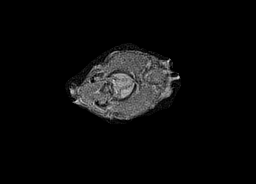
\includegraphics[width=\textwidth]{figures/cs12.png}
    \caption*{a)}
    \end{minipage}
    \begin{minipage}[t]{0.32\textwidth}
    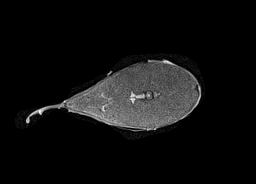
\includegraphics[width=\textwidth]{figures/cs62.png}
    \caption*{b)}
    \end{minipage}
    \begin{minipage}[t]{0.32\textwidth}
    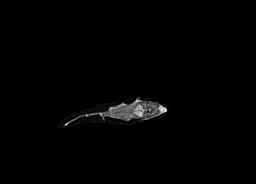
\includegraphics[width=\textwidth]{figures/cs114.png}
    \caption*{c)}
    \end{minipage}
    \caption{Cross-sections from MRI-data: \textbf{a)} close to fish's head (12 mm caudal to head), \textbf{b)} close to fish's transverse plane (62 mm caudal to head, 66 mm cranial to tail), \textbf{c)} close to fish's tail (14 mm cranial to tail). The fish had a total length of 128 mm.}
    \label{fig:crosssections}
\end{figure}

Following from these varying forms, one needs a function describing an ellipsis as its basic form and a factor that defines the tail's shape. Again, we want it to be in parameterised form to define the cross-section relative to the point on the backbone depending on the angle $\varphi$. Hence, we use the parameterised form of an ellipsis and add a factor close to the parameterised Lorenz curve to it. Taking all that into account, we get:

\begin{flalign}
r(\varphi) = \sqrt{\frac{a^2 b^2}{a^2 \cdot cos^2(\varphi) + b^2 \cdot sin^2(\varphi)}} + \frac{m}{(\varphi - \pi)^2+2}.
\label{eq:ellipsis}
\end{flalign}

$r(\varphi)$ specifies the distance from the origin at angle $\varphi$. With different values of $a$, $b$ and $m$ it is then possible to approximate the contours of the individual cross-sections.

\cleardoublepage
\chapter{Data Acquisition and Preprocessing}
    \label{MRIdata}
Before being able to model the cross-sections, reliable anatomical data is needed to base the exact shape on. The way we chose to get the described data is magnetic resonance imaging (MRI). This chapter first sets out the details of the acquisition of the MRI data to then give details about the pre-processing that has been done in order to be able to apply the theoretical model described in the previous chapter.


\section{Acquisition}
    \label{MRI}

For magnetic resonance imaging, we acquired a recently expired but undamaged specimen. The animal was killed for a procedure the preceding day and has been stored refrigerated in partially distilled water. The MRI data was acquired using a 3T clinical scanner (Prisma Fit, Siemens Healthineers AG, Erlangen, Germany) equipped with a flexible 4-canal wrapped-around coil (Flex Small, Siemens Healthineers AG, Erlangen, Germany) and a maximal gradient strength of 80 mT/m. Applying the spin-echo technique, we could get two types of sections useful for modelling purposes: paramedian and paratransverse sections. Paramedian pictures were created using a field-of-view (FOV) of $192 \times 36 \times 24$ mm and a resolution of $0.3 \times 0.3 \times 0.6$ mm, paratransverse pictures with a FOV of $38 \times 27 \times 128$ mm and a resolution of $0.15 \times 0.15 \times 1$ mm. Examples of both types are illustrated in Figure \ref{MRIpic}.

The paramedian pictures are not informative for the shape of the cross-sections but rather give an idea about the location of the backbone, the spinal chord and the electric organ. The latter is placed within the marked red box in Figure \ref{paramedian} while the backbone, detectable by the repeated changes between dark and bright, is located dorsal to it inside the yellow box. In the paratransverse sections the backbone is visible until the cranial end of the swim bladder. Still, in the paramedian picture it cannot be detected till this point. That is why it is only marked until where it is visible in the paramedian data. The pairic structure of \textit{A. Leptorhynchus'} electric organ results from its neurogenicity \cite{bennett1971electric} that is unique for this species, as far as we know. Even further dorsal to the backbone, one can find the spinal chord not clearly visible in the depicted paramedian section, though. The illustrated cross-section on the contrary shows the spinal chord marked in blue quite well. 

\begin{figure}
\begin{tcolorbox}
\centering
\begin{subfigure}[b]{1\textwidth}
    \centering
   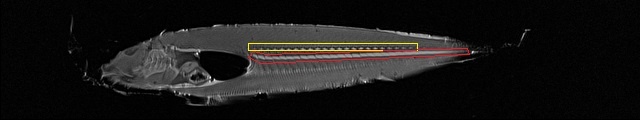
\includegraphics[width=1\linewidth]{figures/coronal_marked.jpg}
   \caption{}
   \label{paramedian} 
\end{subfigure}

\begin{subfigure}[b]{1\textwidth}
    \centering
   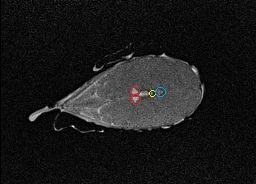
\includegraphics[width=0.5\linewidth]{figures/transverse_marked52.jpg}
   \caption{}
   \label{paratransverse}
\end{subfigure}
\end{tcolorbox}

\caption{MRI data from \textit{Apteronotus Leptorhynchus}. The electric organ is marked in red, the fish's backbone in yellow, and the spinal chord is marked in blue. \textbf{a)} Paramedian section close to the median plane (20 mm from the fish's left). \textbf{b)} Paratransverse section located caudal to the swim bladder (52 mm caudal to the fish's head).}
\label{MRIpic}
\end{figure}

A procedural error in specimen transition to the final measurement configuration lead to artifacts induced by
residual water in the plastic container. This noise is visible in Figure \ref{paratransverse} as grey points or lines around the cross-section itself. Its color made image processing without editing impossible as edge detection has been one of the first necessary steps in that process and the noise was detected as edges as well. Hence, preprocessing of the MRI-cross-sections has been done in form of removing all grey pixels around the fish's body. As this has been executed by hand, it may have led to some inaccuracies in the outer contour of the cross-sections because fish and bag are not always clearly distinguishable. Another consequence was the exclusion of the first eight sections from the editing and thus from the whole modelling process, because bag and fish were not to be distinguished.

Furthermore, the backbone's position needed to be marked in the MRI pictures to be later able to parameterise the cross-section's position relative to it. That was done via coloring the pixels considered as being located inside the backbone in fullwhite by hand, as well. Due to time limits this editing process has only been applied to half of the cross-sectional MRI data. Additionally, we evaluated 60 pictures as being an exact enough basis for later regressions and approximations.

\section{Preprocessing}
    \label{preprocessing}
    
To parameterise the single cross-sections as described in section \ref{Cross sections}, it is obligatory to first determine each contour's distance to the backbone depending on the point on the backbone $l$ and the angle $\varphi$. This can only be done after having transformed and edited the MRI data in various ways. The steps we have executed in order to calcute the mentioned distances are explained in the following paragraphs. 

As a first step, the edited MRI cross-sections were imported into the python project as grey-scale images. To exclude all unneccessary remaining noise outside the fish's contour, a canny edge detection \cite{canny1986computational} has been executed. It uses a smoothed version of the picture by applying Gaussian filters of different widths to it to then compare the intensity changes between pixels. If the gradient magnitude of a pixel is larger than the surrounding pixel's magnitude in direction of the highest intensity change, the pixel is considered an edge \cite{ding2001canny}. We used the canny function from the OpenCV library \cite{opencv_library} to execute the described steps. The marked backbone points cannot be distinguished from other points anymore as points in the edge image are only described by their position not by color. Therefore, the position of the backbone per section, $r$, was determined beforehand by searching for all fullwhite pixels and then taking the average in median and horizontal direction.

Without the outer noise, a convex hull image for each section was created using the convex hull image function from the scikit-image package \cite{scikit-image}. An example of a resulting convex hull can be seen in Figure \ref{fig:convexhull}. The convex hull specifies the cross-section's form quite well because of its elliptic form including just one sharper tip at the bottom. This form does not include any characteristics that can possibly get lost when reducing the information to a convex hull. What is missing in the convex hull image, though, is the backbone point $r$. As this information is highly relevant later on, $r$ needs to be included. One way to do this, is to simply add $r$ as a black point into the convex hull image because the convex hull is represented by white points and a black point will be detected as an edge in the next step. With that, the information about the backbone's position is conserved.

\begin{figure}
    \centering
    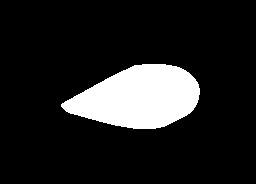
\includegraphics[width = 0.5 \textwidth]{figures/Convexhull68.png}
    \caption{Convex hull created with the canny edge detector function applied to a MRI cross-section that has been edited to remove noise outside the fish. }
    \label{fig:convexhull}
\end{figure}

As mentioned, another edge detection has been applied to the convex hull image because not the interior of the convex hull is relevant in our case but just its outer contour.

In the next step, the position of the backbone has been identified and the point itself has been excluded from the data points of the cross-section. A visualization of the resulting points for one single section can be seen in Figure \ref{fig:contours}. 
\begin{figure}
    \centering
    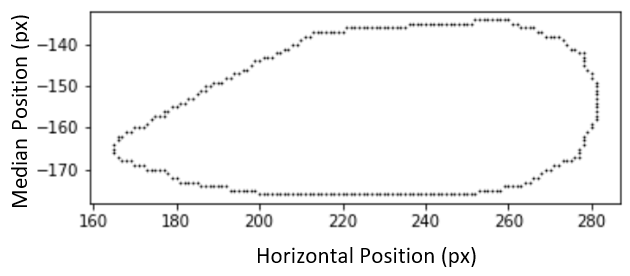
\includegraphics[width = 0.7\textwidth]{figures/contours_tight.PNG}
    \caption{Data points of the outer contour of a cross-section after having determined the convex hull without outer noise and having applied a canny edge detector to the result. }
    \label{fig:contours}
\end{figure}

The contour is still not exactly what we need for defining the distance of its points depending on $\varphi$ and the given cross-section and hence its location on the backbone. The whole contour is turned slightly because the fish was not positioned perfectly straight inside the MRI scanner. Thus, the points are turned slightly and the angle is not what one would expect. To erase this deviation from the optimal position, a rotation needs to be executed. The way to determine the angle for that same rotation is based on the first steps of a principal component analysis (PCA). The reason for applying a PCA is normally the reduction of dimensions by getting rid of dimensions that are not highly informative. To achieve this, a projection from a higher dimensional space to a lower dimensional space is executed such that the variance of the projected points is maximal \cite{scriptLuxi}. We do not want to reduce dimensions in our data but rather find the principal components and the corresponding eigenvectors to approximate the fish's original axes. Obviously, a rotation does not account for a curved axis and that is probably the case in our MRI data. But still, it is a better approximation of the original fish if we rotate the points. Furthermore, in the fitting of the function to the contours the resulting asymmetry gets wiped out because of the function's symmetry. Therefore, we follow the first three steps of the PCA described by \citeA{scriptLuxi} to be able to rotate the contour's points accordingly. 

Primarily, the data points $p_1, p_2, ..., p_n \in \mathbb{R}^2$ have been centered by computing 
\begin{flalign}
\tilde{p_i} = p_i - \overline{p}
\end{flalign}
for $0 < i \leq n, i \in \mathbb{N}$ separately for each cross-section with $\overline{p}$ describing the average over all points.

Secondly, one computes the data matrix $X$ that has the centered data points as rows and in our case the dimension $n \times 2$. The covariance matrix $C$ then follows when calculating the dot product of $X$ with its transpose:
\begin{flalign}
C = X^T \cdot X
\end{flalign}
with $C$ of dimension $2 \times 2$. 

Calculating the eigenvectors of the covariance matrix then leads us to what we wanted: two eigenvectors that approximate the fish's main axes (depicted in Figure \ref{fig:eigenvectors}).

\begin{figure}
    \centering
    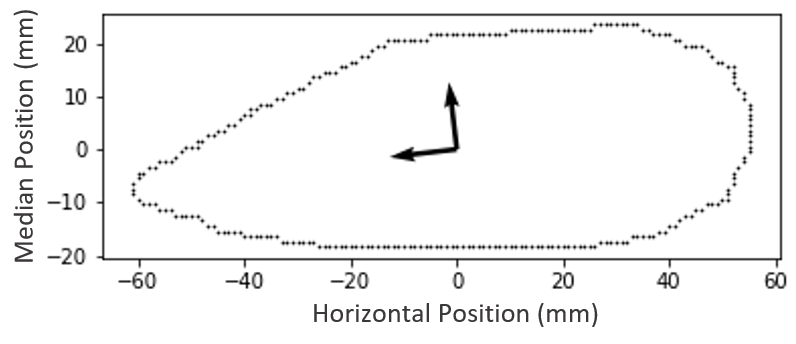
\includegraphics[width = 0.7\textwidth]{figures/eigenvectors.PNG}
    \caption{The figure shows the centered data points of the same section as are depicted in Figure \ref{fig:contours}. Additionally, the normalized eigenvectors of the covariance matrix and resulting from that the approximated fish's original axes, are marked as black arrows. }
    \label{fig:eigenvectors}
\end{figure}

As a next step, the angle $\alpha$ between the eigenvector with the larger eigenvalue, $\vec{e}$, and the horizontal axis $\vec{h}$ is calculated via 
\begin{flalign}
\alpha = \cos^{-1}\left( \frac{\vec{e} \cdot \vec{h}}{||\vec{e} \cdot \vec{h}||} \right).
\end{flalign}

Each point gets rotated around that same angle $\alpha$ in clockwise direction by applying
\begin{flalign}
\Tilde{p_i} =
\begin{pmatrix}
\cos{(-\alpha)} & -\sin{(-\alpha)}\\
\sin{(-\alpha)} & \cos{(-\alpha)}
\end{pmatrix}
\cdot \tilde{p_i}.
\end{flalign}

Having calculated these rotated points, the pre-processing of the MRI data is complete and the basis for fitting edited ellipses to the cross-sections has been created.
\cleardoublepage
\chapter{Implementation Details}
    \label{implementation}

After having transformed the acquired data into a usable format, the fish's anatomy can be modelled. The whole implementation process was done in python \cite{van1995python} using version 3.7.0. The details of that implementation process are explained in this chapter. First, a simplex optimisation was applied to the parameters describing the edited ellipses that approximates the ellipses. Subsequently, the backbone and its relative position to the created cross-sections were defined depending on the fish's curvature. Once this information was gained, a polynomial regression was applied to the parameters describing the cross-sections contours. This process is described in the third section followed by a description of the resulting final function. That same function classifies points according to their position relative to the fish.

\section{Simplex Optimisation on Cross-sections}
    \label{simplex}
    
In order to fit the function described in equation \ref{eq:ellipsis} to the cross-section contours resulting from the transformations in the previous section, an appropriate optimisation method is needed. As the simplex optimisation method \cite{nelder1965simplex} does not assume any premises and works with higher amounts of free variables and nonlinear problems, this is the method we used to find the optimal parameter values for $a,b$ and $m$ for each section. 

As a starting point, the simplex downhill method for unconstrained problems needs $n+1$ points in $n$-dimensional space to form a convex combination of these points. In our case, $n$ is 3 because of the three variables $a,b$ and $m$ that need to be optimised. The point's convex combination is called simplex and gives the method its name. One step is executed by first evaluating all points according to a given error function which is meant to be minimized. For our problem, the error function is based on the distance from the origin to a point on the contour with angle $\varphi$, let us name it $d(\varphi)$. This value is then compared to the fitted value with given parameters $a,b$ and $m$ in $r(\varphi)$ (see equation \ref{eq:ellipsis}) for all existing points and the corresponding $\varphi$-values:
\begin{flalign}
err(a,b,m) = \sum_{all \textit{ } \varphi}{\abs{d(\varphi)-r(\varphi)}}.
\end{flalign}

The next step in the optimisation process is to choose the point for which $err(a,b,m)$ is highest, meaning that this point, let it be called $p_0$, is the worst choice of parameters. $p_0$ therefore gets replaced by a new point $p_{new}$ that is created by projecting $p_0$ through the center of the hyperplane spanned by the other points to the other side. A new simplex with a convex combination of the new point and the remaining old points is the result. This process is repeated until the error function converges indicating a local or global minimum. 

To reduce the probability of ending in a local minimum, we applied the simplex algorithm implemented in the scipy-package \cite{2020SciPy-NMeth} ten times with random starting values (in given intervals: $a \in [-50,50], b\in [-50,100], m \in [-20,20]$) for the first section. The intervals were chosen after manual tests with various starting values whose maximal and minimal values are included in this range. After having found parameter values minimizing the error for the first section, these values were passed over to the next call of the simplex function for the following section and so on. This repeated passing over has been done because we assumed that the optimal parameters do not change a lot between consecutive sections. 

The overall squared error, meaning the added error over all sections (60), was 63,244,722 px$^2$ which is a mean squared error of $1026.68$ px$^2$ per section. One example of a fitted cross-section and the corresponding cross-section points can be seen in Figure \ref{fig:fitted_ellipsis}. Figure \ref{fig:ellipses} assembles the fitted cross-sections in three dimensions to give a better impression of the resulting fish.

\begin{figure}
    \centering
    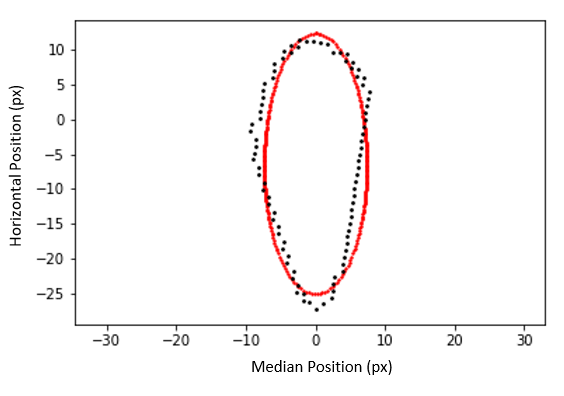
\includegraphics[width = 0.75\textwidth]{figures/FittedEllipsis_64.png}
    \caption{Depicted in red are the fitted cross-section's contour to the cross-section's transformed MRI data (points in black) of a section positioned relative close to the center of the fish's long axis (64 mm caudal to the fish's head). The points in this figure have already been centered on the backbone's position. How this was done exactly is described in chapter \ref{Backbonecoordinates}. One can see clearly, that the tipped edge at the ventral side in the original data is not approximated well by the fitted ellipsis and this holds for all pictures including a tipped edge. }
    \label{fig:fitted_ellipsis}
\end{figure}

\begin{figure}
    \centering
    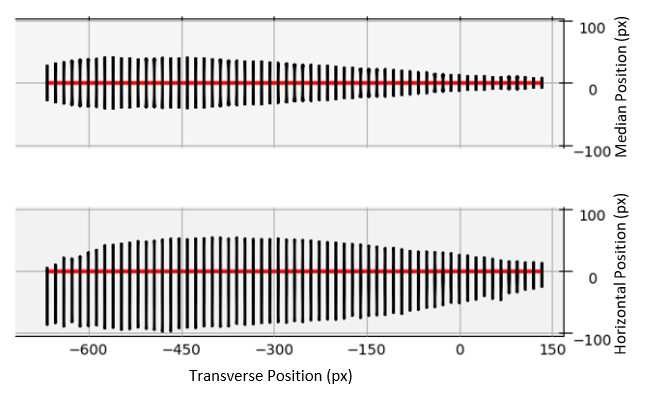
\includegraphics[width = 1\linewidth]{figures/Ellipses.PNG}
    \caption{Ellipses resulting from simplex optimisation (in black) positioned next to each other along the backbone (in red), once as seen from above the fish (upper figure), once as seen from beside the fish (lower figure).}
    \label{fig:ellipses}
\end{figure}


\section{Backbone Coordinates}
    \label{Backbonecoordinates}

To be able to transform the sections from two to three dimensions, the implementation of the backbone itself needs to be done. 

The implementation of the hyperbola modelling the backbone is done straightforward from the mathematical model described in chapter \ref{BackboneModelling}. $f(x)$ is implemented, depending on $\theta$, the angle between x-axis and the second asymptote, and $d$, the intersection with the $y$-axis. 

However, the calculation of $s^{-1}(l)$ cannot be done easily as $s(x)$ is not always a strict monotonic function (for negative $x$-values the curve is a constant function with $y=0$ for most $\theta$ and $d$ values). However, strict monotony would be necessary for building the inverse function. Therefore, the calculation of $s^{-1}(l)$ is replaced by a look-up table with 10000 entries ($x \in [Head, Head + 120]$, $l \in [0, s(Head+120)]$). Searching for a given $l$ in that same look-up table results in a value close to the exact inverse value, $s^{-1}(l)$. The search is done via a binary search that has a running time of $O(log(n))$ with $n$ being the number of entries in the look-up table. 

As the next step, the cross-sections need to be positioned correctly relative to the now existing backbone-coordinates. Therefore, the contours are supposed to be centered around the backbone's position and not around its center of mass like previously. Hence, a translation in horizontal directions needs to be executed according to each section's position relative to the backbone. 

As described in chapter \ref{preprocessing}, the coordinates of the backbone have been included in the convex hull picture and could therefore be determined later on in the second edge image. Its median coordinate is not relevant because of the fish's symmetry in median direction. In contrast, the horizontal coordinate is the source used to determine the necessary translation called \textit{x\_offset} in the further descriptions and also in our code (see supplementary material). A translation for the determined sections could be done easily with the detected backbone positions, but only for the discrete positions on the backbone at which the sections are located and only for sections located caudal to the swim bladder. However, we need to be able to calculate the \textit{x\_offset} at each point $l$ on the backbone. Thus, a polynomial regression with a degree of two was applied to the detected positions to predict the missing positions. The $R^2$ value for that model is 0.95 and is thus providing a sufficient fit. The model is depicted in Figure \ref{fig:paramreg} at the right bottom.

The backbone's positions can be approximated for any $l$ with the resulting function. Hence, the fitted contours can be positioned relative to the backbone in the two-dimensional space.

\section{Ellipses Parameter Regression}
    \label{parameterregression}
    
Additionally to the polynomial regression for the \textit{x\_offset}, polynomial regressions were applied to the parameters $a,b$ and $m$ which resulted from the simplex optimisation. The reason for these additional regressions are the jumps that can be seen in Figure \ref{fig:fitted_ellipsis} that may be caused by inaccuracies in previous transformation steps. $a$ and $b$ are well predictable with a polynomial regression of degree 3 as their $R^2$ values are 0.99 and 0.93, accordingly. In contrast, $m$, the parameter for defining the contour's tip at the bottom, does not seem to be describable by a polynomial model, at least not with degree 3 ($R^2 = 0.46$). But even with a degree of ten, the fit does not get significantly better. All those regressions are depicted in Figure \ref{fig:paramreg}. 

The resulting smoothed fish in three dimensions is visualized in Figure \ref{fig:ell_regression}.

\begin{figure}
\centering
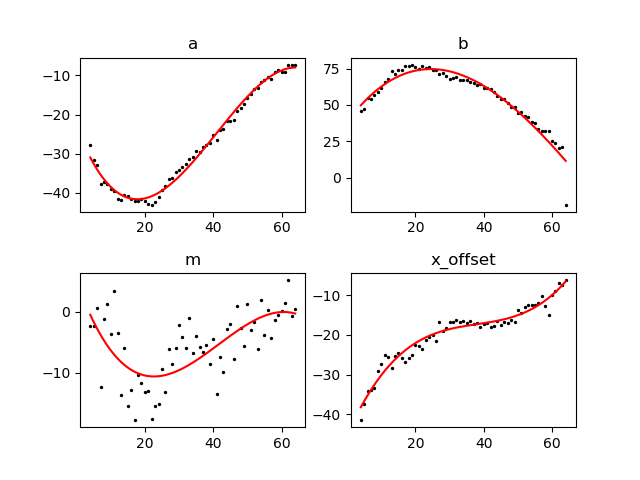
\includegraphics[width = 1\linewidth]{figures/param_regressions.png}
\caption{The four figures show the values for $a,b,m$ and the \textit{x\_offset} given by simplex optimisation for the existing cross-sections from the MRI data (points in black). The red lines each show the results of the polynomial regressions with degree 3 over the fitted values separately for $a,b,m$ and the \textit{x\_offset}.}
\label{fig:paramreg}
\end{figure}

\begin{figure}
\centering
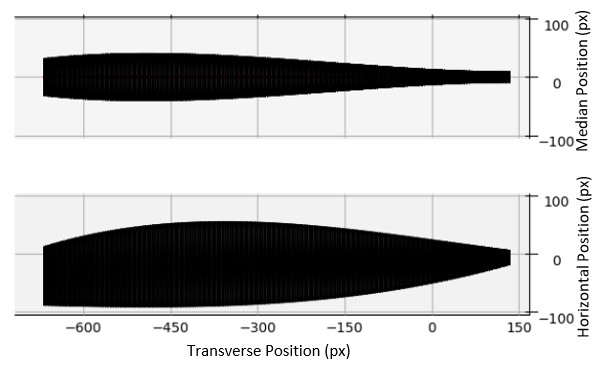
\includegraphics[width = 1\linewidth]{figures/Ellipsis_regression.png}
\caption{Smoothed ellipses with parameters $a$,$b$,$m$ and  $x\_offset$ resulting from the polynomial regressions over each parameter put together along the backbone to form the fish's body. The upper picture shows the resulting fish's contour as seen from above the fish, the picture at the bottom as seen from aside.}
\label{fig:ell_regression}
\end{figure}


\section{Fish-discrimination Function}
    \label{finalfunction}

The purpose of the final function is to describe a point's position relative to the fish. Is the point located outside the fish or inside? If the latter is the case: is it positioned within the backbone, the spinal chord or the electric organ? These five categories should be distinguished from each other to then be able to model the fish's electric field and the response of its electroreceptors precisely. \\

\subsection{Definition of the Closest Point}
    \label{closestpoint}
The first step towards a categorization of a point $p_W$, given in world coordinates, is calculating the point $l$ on the backbone to which $p$ has the smallest distance. To do so, the following distance function is defined based on the backbone's definition. $P$ is the point for which its position needs to be determined, $P_B$ is a point on the backbone described only by the $x-$coordinate.

\begin{flalign}
||P-P_B|| = \sqrt{(p_x-x)^2 + (p_y-\frac{1}{2}(ax + \sqrt{4d^2 + a^2x^2})^2 + p_z^2}
\end{flalign}

The distance function depends solely on $x$ and therefore one can take its derivative and set it to zero to get the $x$-value for which it is minimal, $x_0$. This was done in python using the sympy differentiation and solve methods \cite{sympy2017}. Having evaluated $x_0$, the calculation of $l$ follows straightforward from \ref{eq:s_x}.

The tangential vector of $l$, described as $\vec{e_1}$ in previous paragraphs, is then orthogonal to the vector between $l$ and $p$ because the orthogonal distance is always smaller than non-orthogonal distances \cite{ahn2002orthogonal}. Points having their closest point $l \not \in [0,120]$ can be directly labeled as outside the fish as long as the bent of the fish's tail is not positioned very close to the tail's endpoint. If that happens, it may lead to a corresponding point $l$ cranial to the fish's tail while another perpendicular point $l_0$ is positioned caudal to the tail although it is further away. Still, it would then be possible that the point to be categorized is localized within the fish, because the distance to $l_0$ is smaller then the threshold at this point. The described position of the fish with a bent of the tail really at the end of the fish is not something that is interesting for research purposes. As described in section \ref{BackboneModelling}, the standard exploration behaviour is executed with a bent approximately at the fish's center close to the transverse section. The boundaries for points being possibly inside or definitely outside the fish, are depicted in Figure \ref{fig:borders}.

The orthogonality property for points being possibly inside the fish has been used to test the result from the calculations so far via the scalar product. For 150 tested points the maximal scalar product was 0.0688. It is not exactly zero because of inaccuracies following from the look-up table evaluating $s^{-1}(x)$.

\begin{figure}
    \centering
    \includesvg[width = 0.85\linewidth]{figures/outer_borders.svg}
    \caption{Points being labeled as inside or outside the fish according to the illustrated boundaries. The figure shows the fish's backbone in a curved position (black line; $\theta = 60, d = 4, Head = -70$) from head to tail and its theoretical further development before the head and behind the tail (dashed lines). The outer boundaries (dotted lines) determine whether points are possibly inside the fish or outside, at this point not depending on their distance to the backbone but only on their corresponding point $l$ on the backbone which has the closest distance to the given point. Points to the left of the left boundary do have a closest point $l$ on the backbone smaller than $0$, points to the right of the right boundary fulfil $l>l(Tail)$. The bend of the right border is caused by the bend of the backbone because points located higher than the border's bend possibly have two points on the backbone with an orthogonal tangential vector. One then needs to distinguish between the points being closer and further away and that is done according to the vertical part of the right border.}
    \label{fig:borders}
\end{figure}


\subsection{Relative Position to the Fish}
    \label{relativeposition}
Having calculated the closest point $l$ on the backbone, the next step for determining $p$'s position is getting its position relative to that same point l. To achieve this, one needs to transform ${}^Wp$, given in world-coordinates, by ${}^LT_W$, where $L$ describes the coordinate frame centered on $l$. Therefore, the inverse of ${}^WT_L$ needs to be calculated and then multiplied with $p$. It is
\begin{flalign}
{}^WT_L = \begin{pmatrix} cos(\varphi) & -sin(\varphi) &0 & l_x \\
sin(\varphi) & cos(\varphi) & 0 & l_y \\
0&0&1&0 \\ 0&0&0&1\end{pmatrix}
\end{flalign}
with
\begin{flalign}
\varphi = cos^{-1}\left(\vec{e_1} \cdot \begin{pmatrix}
1 \\ 0 \\ 0 
\end{pmatrix}\right).
\end{flalign}
No normalization is needed here, because both $\vec{e_1}$ and the $x$-axis unit vector do have a norm of 1.
Calculating the inverse of that matrix and applying it to ${}^WP$ results in:
\begin{flalign}
{}^LT_W \cdot {}^WP = \begin{pmatrix} cos(\varphi) & sin(\varphi) &0 & -l_x\cdot cos(\varphi) - l_y \cdot sin(\varphi) \\
-sin(\varphi) & cos(\varphi) & 0 & l_x \cdot sin(\varphi) -l_y\cdot cos(\varphi) \\
0&0&1&0 \\ 0&0&0&1\end{pmatrix}
\cdot
\begin{pmatrix}
p_x \\ p_y \\p_z \\1
\end{pmatrix}
= {}^LP.
\end{flalign}

Then ${}^LP$ is of the form
\begin{flalign}
{}^LP= \begin{pmatrix}
\tilde{p_x} \\  \tilde{p_y} \\ p_z \\1
\end{pmatrix}
\label{eq:l_p}
\end{flalign}

with

\begin{flalign}
\tilde{p_x} = (p_x-l_x) \cdot cos(\varphi) + (p_y - l_y) \cdot sin(\varphi) \\
\tilde{p_y} = (l_x-p_x) \cdot sin(\varphi) - (l_y-p_y) \cdot cos(\varphi).
\label{eq:py}
\end{flalign}

The tangential vector $\vec{e_1}$ of $l$ can be written as

\begin{flalign}
\vec{e_1}=\begin{pmatrix}
cos(\varphi) \\ sin(\varphi) \\ 0
\end{pmatrix}
\end{flalign}

$\vec{lp}$ by definition is

\begin{flalign}
\vec{lp} = \left(\vec{p} - \vec{l}\right) = \begin{pmatrix}
p_x - l_x \\ p_y - l_y \\ p_z - l_z
\end{pmatrix}.
\end{flalign}

Because of the perpendicular arrangement of $\vec{e_1}$ and $\vec{lp}$, it holds

\begin{flalign}
\langle \begin{pmatrix}
p_x - l_x \\ p_y - l_y \\ p_z - l_z
\end{pmatrix},
\begin{pmatrix}
cos(\varphi) \\ sin(\varphi) \\ 0
\end{pmatrix}
\rangle = 0
\iff (p_x - l_x) \cdot cos(\varphi) + (p_y - l_y) \cdot sin(\varphi) = 0.
\end{flalign}

As this is equivalent to $\tilde{p_x}$, the $x$- coordinate of ${}^LP$ is always zero. $p_z$ does not change, as $l_z$ is always zero. Following from that, there is no translation in $z$-direction no matter the exact values of $p$. That results in

\begin{flalign}
{}^LP= \begin{pmatrix}
0 \\ \tilde{p_y} \\ p_z
\end{pmatrix}.
\end{flalign}

To be able to decide, whether $p$ is located inside the fish, one needs to compute the threshold for the resulting angle between ${}^LP$ and the origin. The fitted ellipses were constructed not relative to the position of the backbone but to the backbone translated by the corresponding \textit{x\_offset}, let us name that point $b_0$. Therefore, the angle and distance of ${}^LP$ need to be calculated relative to $b_0$, as well. Translating $p$ by the \textit{x\_offset} and then calculating both values has the wanted effect. Hence, this is what has been done:
\begin{flalign}
d_p &= \sqrt{\tilde{p_y}^2 + (p_z +x\_offset)^2}\\
{}^L\tilde{P} &= \begin{pmatrix}
\tilde{p_y} \\ p_z + x\_offset
\end{pmatrix}, \vec{e_x} = \begin{pmatrix}
1 \\ 0 
\end{pmatrix}\\
\theta &= cos^{-1}\left( \frac{{}^L\tilde{P}\cdot \vec{e_x}}{||{}^LP'\cdot \vec{e_x}||}\right).
\end{flalign}

Using the coefficients from the parameter regression described in section \ref{parameterregression}, it is possible to calculate the exact parameters for the determined $l$-value. Substituting these parameters and the angle $\theta$ into equation \ref{eq:ellipsis} leads to the distance from $b'$ to the point on the contour with the same angle. Thus, this value specifies the threshold for categorizing a point as inside or outside the fish. Comparing this threshold to $d_p$, the categorization inside/outside is complete. The fish resulting from all points being labeled as inside can be seen in Figure \ref{fig:final_fish}.

\begin{figure}[ht] \label{ fig7} 
\captionsetup[subfigure]{labelformat=empty}
  \begin{subfigure}[b]{0.5\linewidth}
    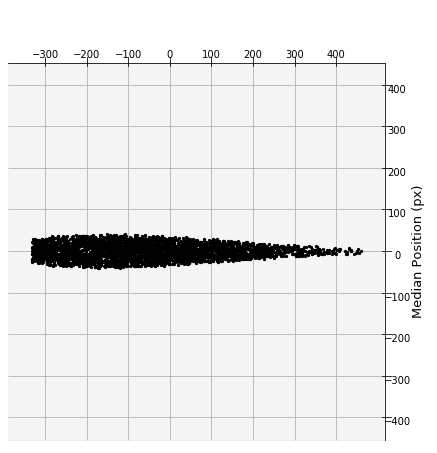
\includegraphics[width = 1 \linewidth]{figures/final_fish_straight_median.PNG} 
  \end{subfigure} 
  \begin{subfigure}[b]{0.5\linewidth}
    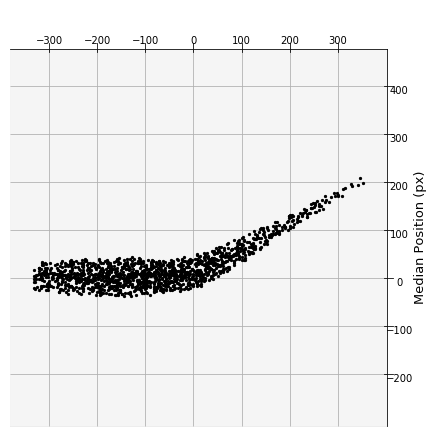
\includegraphics[width = 0.99 \linewidth]{figures/final_fish_turned_median.png} 
  \end{subfigure} 
  \begin{subfigure}[b]{0.5\linewidth}
    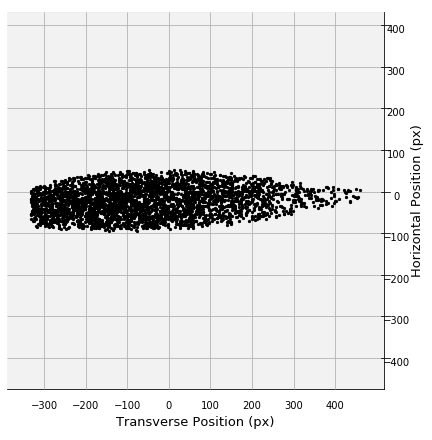
\includegraphics[width = 1\linewidth]{figures/final_fish_straight_horizontal.PNG} 
  \end{subfigure}
  \begin{subfigure}[b]{0.5\linewidth}
    %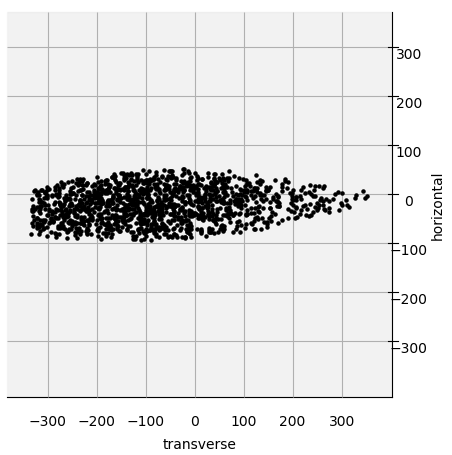
\includegraphics{figures/final_fish_turned_30_2_minus50_10000_1.png} 
    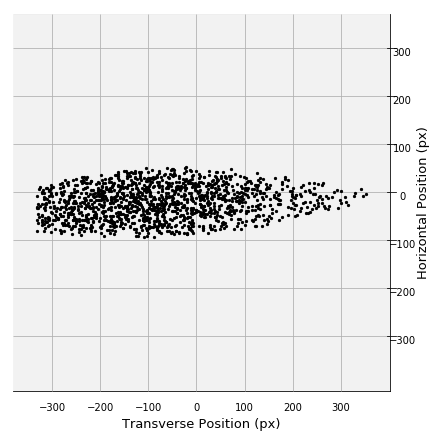
\includegraphics[width = 1.02\linewidth]{figures/final_fish_turned_horizontal.png}
  \end{subfigure} 
  \caption{On the left, one can see all points of 10000 random points within a range of $Head$ to $Tail$ in transverse direction, $-100$ to $100$ in median direction and $-50$ to $50$ in horizontal direction labeled as inside the straight fish ($\theta = 0, d = 0, Head = -50 \cdot (1/0.15)$) by the final function. The top graphic shows the fish as seen from above, the bottom one as seen from aside (see \ref{fig:ell_regression} for comparison). On the right, the same can be seen for a fish with values of $\theta = 30, d = 2$ and $Head = -50 \cdot (1/0.15)$ and 10000 points within the ranges of $Head$ to $Tail$, $-50$ to $220$ and $-100$ to $60$, respectively. Less points are labeled as being inside for the turned fish because the median range is a lot wider than for the straight fish.}
  \label{fig:final_fish}
\end{figure}

\subsection{Categorization within the Fish}
    \label{innerparts}
    
Next, the differentiation of the considered inner parts can be done. This further differentiation is only necessary, of course, for points categorized as being on the inside of the fish. 

First, we want to consider the backbone. Measured on various MRI pictures, the backbone seems to have a constant radius $r_b$ of about $0.415$ mm. It is observable on picture 34 and all pictures caudal to that one. The straightforward classification for points positioned inside the backbone therefore is based on these two criteria: Is the distance of ${}^LP$ (without the translation of \textit{x\_offset}) smaller than $r_b$? And, secondly, is the corresponding $l$ positioned caudal or at the corresponding position of cross-section number 34? 

Second, points located inside the spinal chord should be labeled as such. The radius of the spinal chord, $r_s$, being $0.466$ mm is constant throughout the whole fish. It is also visible in pictures caudal to the $34^{th}$ picture. As it can be seen in Figure \ref{fig:innerparts}, there is no distance between spinal chord and backbone. At least, it is too small to detect in the MRI scan, if present. A translation of the point by $r_s+r_b = 0.881$ mm in ventral direction and a calculation of this point's distance to the origin is equivalent to calculating the point's distance directly to the spinal chord's center. Again, the two criteria need to be fulfilled in order to classify a point as positioned inside the considered part, in this case the spinal chord. 

Third, it needs to be verified if the given point is located within the electric organ or not. As depicted in Figure \ref{fig:innerparts}, the electric organ was modelled by two mirrored triangles ventral to the backbone. The offset between the backbone's center and the triangles' left/right tip is termed \textit{e\_offset} and varies along the backbone. It is visible in a triangular form on the MRI images only in sections 50 and the ones caudal to it. Cranial to that, it is visible until the cranial end of the swim bladder but its form is different. Due to time constraint, this part of the electric organ has not been included into the implementation. For the included part, primarily, one needs to define \textit{e\_offset} and \textit{width}, distance between left and right tip of the electric organ, at each point of the backbone. To do so, two linear regressions were performed using three values at three different section as a basis (one for the \textit{width}, one for the \textit{e\_offset}). The resulting $R^2$ values suggest that the models fit well: $R^2_{width} = 0.9998, R^2_{e\_offset} = 0.9836$. The fitted coefficients and intercepts were then used to define width and e\_offset at each point $l$. The application of the following formulas then leads to the position of the triangles vertices.
\begin{flalign}
\frac{\gamma}{2} &= \sin^{-1}\left({\frac{0.5 \cdot c}{b}}\right) \\
A &= \begin{pmatrix}
\pm 0.5 \cdot width \\ -e\_offset
\end{pmatrix}\\
B &= \begin{pmatrix}
A_x \pm b \cdot \cos\left(\frac{\gamma}{2}\right) \\ A_y -b \cdot \sin\left(\frac{\gamma} {2}\right)
\end{pmatrix}\\
C &= \begin{pmatrix}
A_x\pm \cdot \cos\left(\frac{\gamma}{2}\right) \\A_y +b \cdot \sin\left(\frac{\gamma} {2}\right)
\end{pmatrix}.
\end{flalign}
With that, one can calculate whether a point is positioned within one of the two triangles. One way to do that is to transform the given point into the barycentric coordinate system \cite{farin2008mathematical}. Hence, the point is written as a linear combination of the vertices $A,B,C$: $ P = s \cdot A + t \cdot B + u \cdot C$ with 
\begin{flalign}
s = \frac{area[P, B, C]}{\mathcal{A}}\\
t = \frac{area[P, C, A]}{\mathcal{A}}\\
u = \frac{area[P, A, B]}{\mathcal{A}}
\end{flalign}
 where $\mathcal{A}$ describes the triangle's area and thus $\mathcal{A} = area[A,B,C]$. 
 
 In two dimensions it holds: $s+t+u = 1$, no matter where $P$ is positioned. Additionally, if $P$ is located within the triangle, it follows that $s,t,u \geq 0$. This property can be used to test whether a given point is located within or outside a triangle.
 
The described process was implemented and builds the second condition for a point being located within the electric organ alongside with the point being positioned closest to a point $l$ on the backbone corresponding to a section $\geq 50$. 

\begin{figure}
    \centering
    \fbox{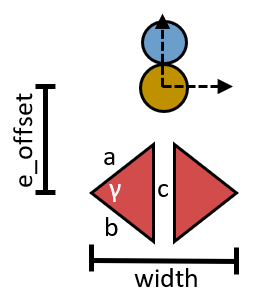
\includegraphics{figures/Crosssectionmodel.PNG}}
    \caption{This illustrations depicts a simplified version of the considered parts in the interior of the fish. The backbone is depicted in yellow below the spinal chord (blue). The electric organ is shown in red, its offset is marked on the left. It is measured from the electric organ's tip to the center of the backbone. The width specifies the width between the two tips of the electric organ.}
    \label{fig:innerparts}
\end{figure}

In conclusion, a given point is label as 'outside','inside', 'backbone', 'spinal chord' or 'electric organ'. The resulting labels for points located closest to the same $l$ is depicted in Figure \ref{fig:sectionlabel}.

\begin{figure}
    \centering
    \includesvg[width = 0.8\textwidth]{figures/labeling_section29.svg}
    \caption{Labeling of 10000 points within a range of $-50$ to $50$ mm on the median axis and $-100$ to $60$ mm on the horizontal axis in the paratransverse section located $58$ mm caudal to the fish's head. Points in red are classified as outside the fish, points in yellow are classified as being on the spinal chord, points on the backbone are depicted in violet and points in green are located within the electic organ. Points classified as inside the fish are not included for enhanced clarity of the inner part labels.}
    \label{fig:sectionlabel}
\end{figure}







\cleardoublepage
\chapter{Discussion and Outlook}
    \label{Discussion}

The aim of this thesis was to model \textit{A. leptorhynchus'} anatomy numerically as accurately as possible. For this purpose, first, a geometrical approach was presented including the modelling of the backbone by a hyperbola, the definition of the normal planes relative to this curve and the approximation of the cross-sections by the sum of parameterized ellipses and a parameterized version of the Lorenz-Kurve. The latter aspect was considered to take into account the tipped form at the ventral side. With MRI data of one fish, the cross-sections' contours were then investigated. The final turned and centered data points were fitted to the tipped, parameterized ellipses via simplex optimization. The resulting parameters could then be smoothed and made continuous by applying a polynomial regression to each parameter. In the last step, the final function was implemented which differentiates between points being on the outside and on the inside of the fish. Additionally, if the latter is the case, points inside the backbone, inside the spinal chord or inside the electric organ are labeled as such.

The underlying mathematical ideas do work to a specific degree of accuracy. Still, there is potential to improve certain details to increase the anatomical closeness of model and fish. First, the hyperbola modelling the fish's backbone is dependent on several parameters. The position of head and tail of course defines the point along the fish's long axis where it is bent. This part seems reasonable because of the fixed body length and with that, it only depends on one parameter: the transverse position of the fish's head. The curvature, in contrast, is defined by $\theta$ and $d$ and these two parameters interact with one another. Therefore, it is hard to predict, which parameter values result in what kind of curvature. This is only a minor disadvantage for the research this model is made for because a very limited amount of different body shapes is necessary. Hence, with a bit of testing, the parameters leading to the wanted shapes can be found. That should be sufficient to draw conclusions about the usefulness of a bending behaviour to explore the environment. If a bent body leads to different electroreceptor's responses, this can be processed in an informative way, one could argue for the fish to use bending behaviour as an aid for electrolocation. A prerequisite for this is, of course, the confirmation of the former observations of this exploratory behaviour. If it turns out, that \textit{A. leptorhynchus} do not bent their tail at all when approaching new objects in their surroundings, the bending feature would be useless for future research. 

The second mathematical factor allowing room for improvement is the function modelling the cross-sections. As the wide spread of the $m$-values over the cross-sections from the simplex optimization indicates, no systematic structure seems to be present with the given function. Additionally, the values are relatively close to zero for the most part. These two factors together lead to the conclusion that the function we have chosen is not optimally suitable for the shape defined by the cross-sections. Even though the value varies from zero and with that, one can be sure that it improves the approximation at least a bit comparing it to a function that includes only a parameterized ellipses. Therefore, the chosen function seems to be partly reasonable but does not suffice to approximate the sections' tip at the ventral side. Thus, searching for alternative functions could turn out as a worthwhile approach to improve the model.

A major mistake that we made was the way we created the MRI data. The fish's wet condition and the wet bag it was surrounded by, led to irritations in the data. In the first step, that led to time-consuming manual image editing that could have been avoided. Because of the amount of time, we chose to only include every second paratransverse section. It is difficult to estimate the influence this decision had on the overall model's accuracy. Still, it is probable that the omission of half of the data decreased the accuracy to some degree. Additionally, the differentiation between pixels belonging to the fish itself and the ones colored in grey due to the wet bag has been done by hand. Of course, we tried to do that as accurate as possible but the possibility of unintentional structural mis-classifications remains. Such a structural mistake would have then been included in the first edge-detection and due to that in all the follow-up steps until the fitting of the ellipses. Using another material to place the fish in could avoid the pre-processing steps and the possibly resulting inaccuracies. Furthermore, placing the fish on something that ensures a straight body position would have been a better choice for the scan. It would have eased the image processing and made the determination of the eigenvectors and the resulting rotation superfluous. 

A further step that could be added to the modeling routine is a detection of the backbone in a more reliable manner. The way we did it, was by marking the pixels we assumed to be belonging to the backbone and then later detecting the markers within the images. The labeling by hand, here again, may have caused inaccuracies or structural mistakes in the image processing. One option to avoid this could be to apply a neural network build to detect certain structures (those networks are for example used to detect single cells in biological research applications). Such a network could then be trained to detect the contours of a backbone in the MRI data. Still, to train the network, labeling by hand would need to be done beforehand and could possibly result in the same structural mistakes. The polynomial regression that has been applied to the \textit{x\_offset} seems like a reasonable starting point to correct at least small mistakes during the marking process.

Another aspect that has not been considered in all its details is the fish's head and tail. They are not fully included in the MRI data or at least cannot be fully used, as is the case for the first eight MRI cross-sections. Therefore, head and tail's form are partly excluded in the model.

Changing the topic to the implementation itself, we conducted some mistakes that do not change the functions behaviour or the correctness of the result but possibly lead to difficulties while trying to understand the code. As this is important when trying to use the model created here for different species of weakly electric fish, we explain them in more detail. In the beginning of the programming phase, we defined the length of the fish as being 120 because that was the amount of usable MRI data that we had. The following regressions were all based on this length. Later on, we realized that the distance between the sections needed to be increased by multiplying the transverse and median coordinates of the corresponding backbone position by $1/0.15$ as this is the ratio to transform pixels into millimeters with our MRI data. That resulted in an obligatory stretching in the final function that may not be obvious for someone who has not been involved in the implementation process. Therefore, the simpler and more understandable way would have been to include the stretching factor right from the beginning. 

Despite the inaccuracies and slight draw-backs mentioned above, the created anatomical model is a lot closer to a real fish's body shape then the models used in former studies. Due to the improved accuracy, one can approximate the fish's electric sensory system in more detail and possibly draw more detailed conclusions. This will be done in the project this thesis is part of. Due to this the anatomical model makes a contribution in answering further research questions about the electric sense accurately. One question that could be addressed, for example, is the varying amount of receptors spread across the fish's body. The anatomical model could allow us to model the electric potentials at each body position exact enough to explain why this distribution could be advantageous for the fish's electrolocation. Additionally, one can test for the reach of the electric sense as this is an important factor for explanations concerning evolutionary benefits. If its reach is relatively low, one cannot argue for it being a replacement system for the visual system when being confronted with a lack of light. There are many more open questions about electroception in need to be investigated. In all of those that can be investigated using an in silico model, the inclusion of an anatomical model leads to an increased reliability in the resulting data. 

The theory of the model is not limited to research about \textit{A. leptorhynchus}. Obviously, this is the case for the implemented model based on the MRI data about this species. Still, one would only need to adapt the preprocessing steps of the MRI data according to the MRI data one wants to use and the function approximating the cross-sections' contours. The rest of the code can be easily transferred and used for research in different species of fish. 

Following this line of research, the approach developed in this bachelor thesis has the potential to prove helpful in gaining knowledge about the electric sense in all weak electric fish, especially in Mormyriformes and Gymnotiformes. Is the active electric sense used for electrolocation or solely for electrocommunication? What is the electric sense's major evolutionary advantage that lead to its probably analogous evolution in two different orders? Those questions may be addressed using an in silico model including an anatomical model of the species under research based on the presented approach. 

%%%%%%%%%%%%%%%%%%%%%%%%%%%%%%%%%%%%%%%%%%%%%%%%%%%%%%%%%%%%%%%%%%%%%%%%%%%%%
%%% Bibliographie
%%%%%%%%%%%%%%%%%%%%%%%%%%%%%%%%%%%%%%%%%%%%%%%%%%%%%%%%%%%%%%%%%%%%%%%%%%%%%

%\addcontentsline{toc}{chapter}{References}

\bibliography{mylit}
\bibliographystyle{apacann}
%% Obige Anweisung legt fest, dass BibTeX-Datei `mylit.bib' verwendet
%% wird. Hier koennen mehrere Dateinamen mit Kommata getrennt aufgelistet
%% werden.

\cleardoublepage

%%%%%%%%%%%%%%%%%%%%%%%%%%%%%%%%%%%%%%%%%%%%%%%%%%%%%%%%%%%%%%%%%%%%%%%%%%%%%
%%% Erklaerung
%%%%%%%%%%%%%%%%%%%%%%%%%%%%%%%%%%%%%%%%%%%%%%%%%%%%%%%%%%%%%%%%%%%%%%%%%%%%%
\hspace*{-4.5cm}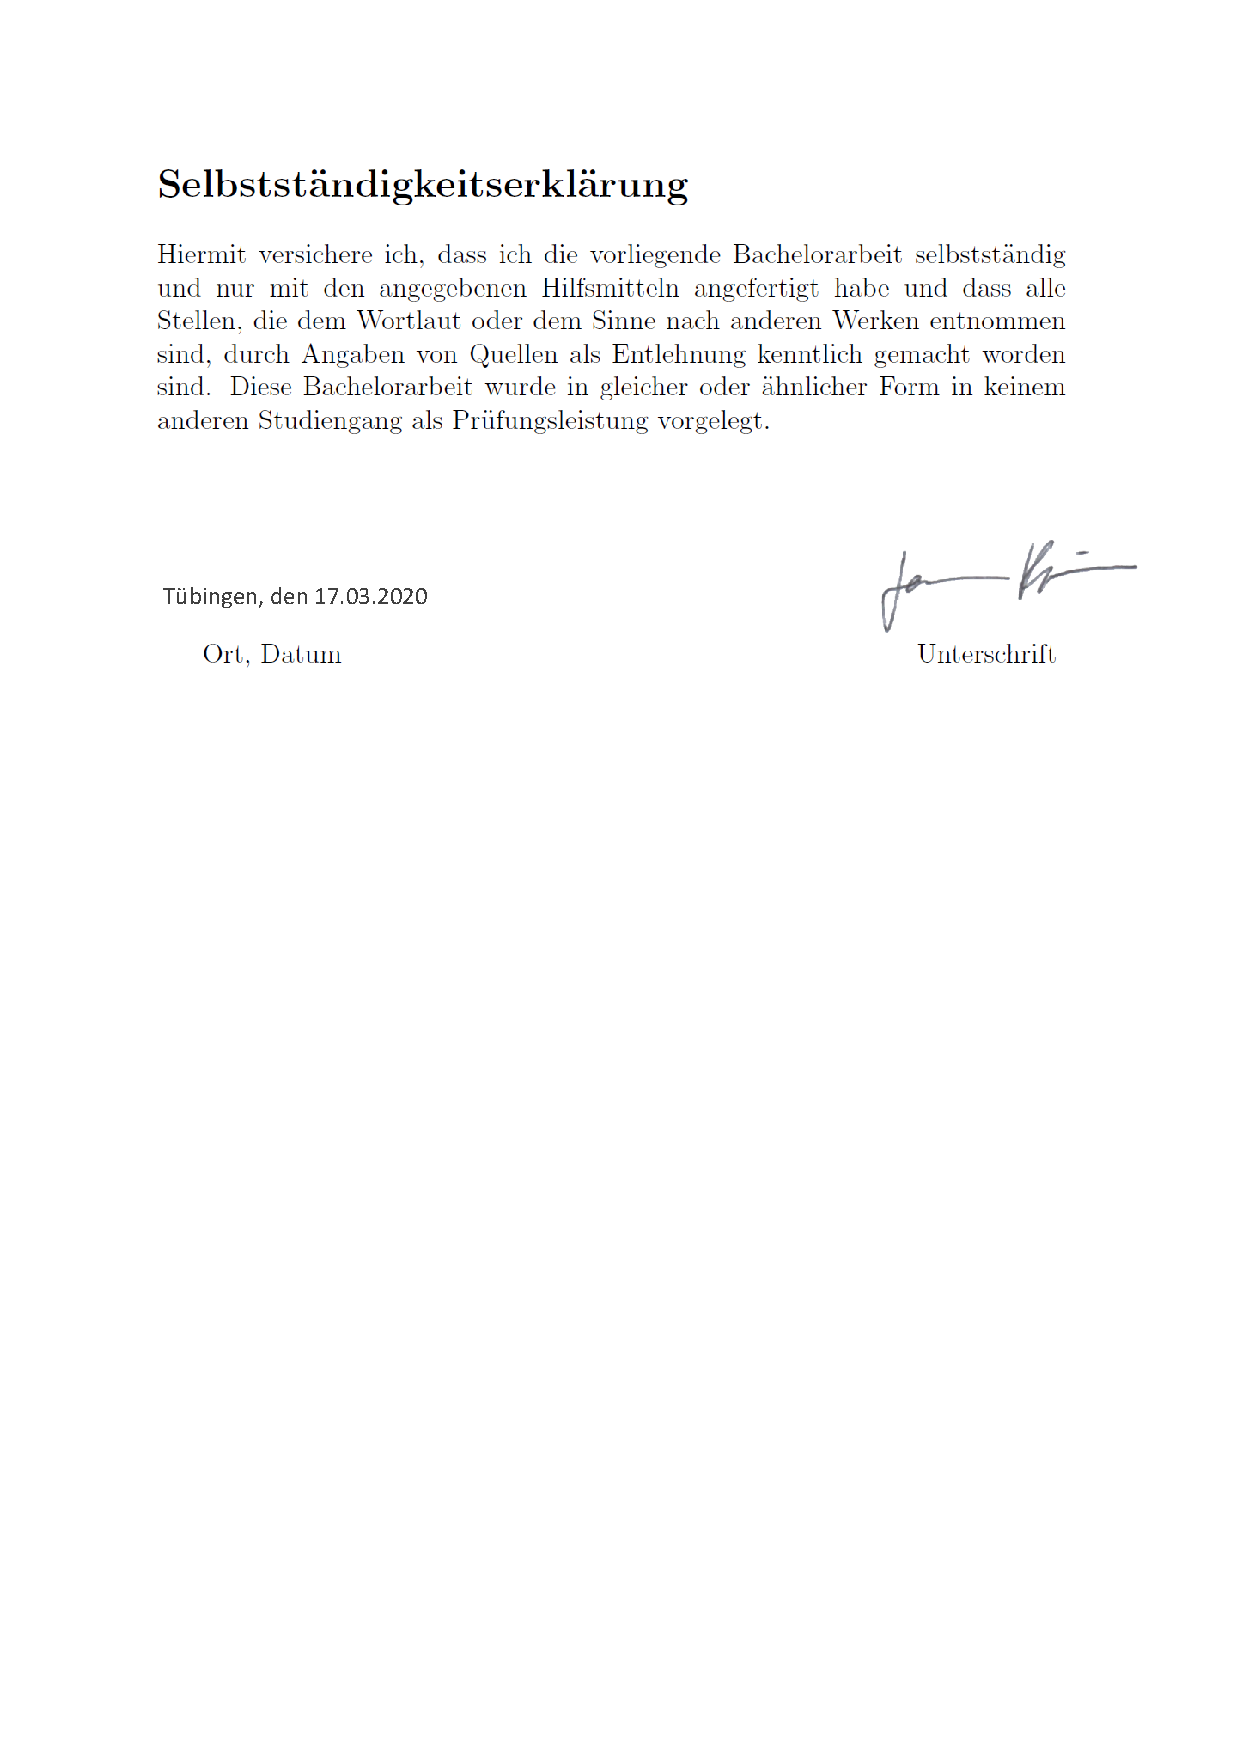
\includegraphics[page = 1]{figures/Selbststaendigkeitserklaerung.pdf}

\end{document}

